\documentclass[12pt, a4paper, oneside]{ctexart}
\usepackage{amsmath, amsthm, amssymb, bm, color, framed, graphicx, hyperref, mathrsfs, float}
\pagestyle{plain}

% multi-column
\usepackage{tasks}
% itemize
\NewTasksEnvironment[label=(\arabic*), label-width=3ex]{exercise}

\everymath{\displaystyle}

\title{\textbf{第一次随堂测试}}
\author{U08M11002 Fall 2023}
\linespread{1}
\definecolor{shadecolor}{RGB}{241, 241, 255}

\newcounter{problemname}
\newenvironment{problem}{\stepcounter{problemname}\par\noindent\textbf{题目\arabic{problemname}. }}{\\\par}
\newenvironment{warning}{\begin{shaded}\par\noindent\textbf{提交作业方式:}}{\end{shaded}\par}

\begin{document}

\maketitle

\hspace{1em}

\begin{problem}
判断 $f(t)  = \cos 2t + 2\sin \pi t$ 是否为周期信号,若为周期信号,求出其周期。
\end{problem}

\begin{problem}
判断 $f(t) = A U(t)\cos (\omega t + \phi)$ 是功率信号还是能量信号。
\end{problem}

\begin{problem}
求 $\int_{-5}^{1}[\delta(t-2)+\delta(t+4)]\cos\frac{\pi}{2}tdt$ 积分。
\end{problem}

\begin{problem}
计算 $\int_{-\infty}^{\infty} \frac{\sin \pi t}{\pi t} \delta(t) dt$
\end{problem}

\begin{problem}
已知信号$f(5-4t)$的波形如下图所示,分别画出$f(t)$和$\frac{d}{dt}f(t)$的波形。
\begin{figure}[h]
	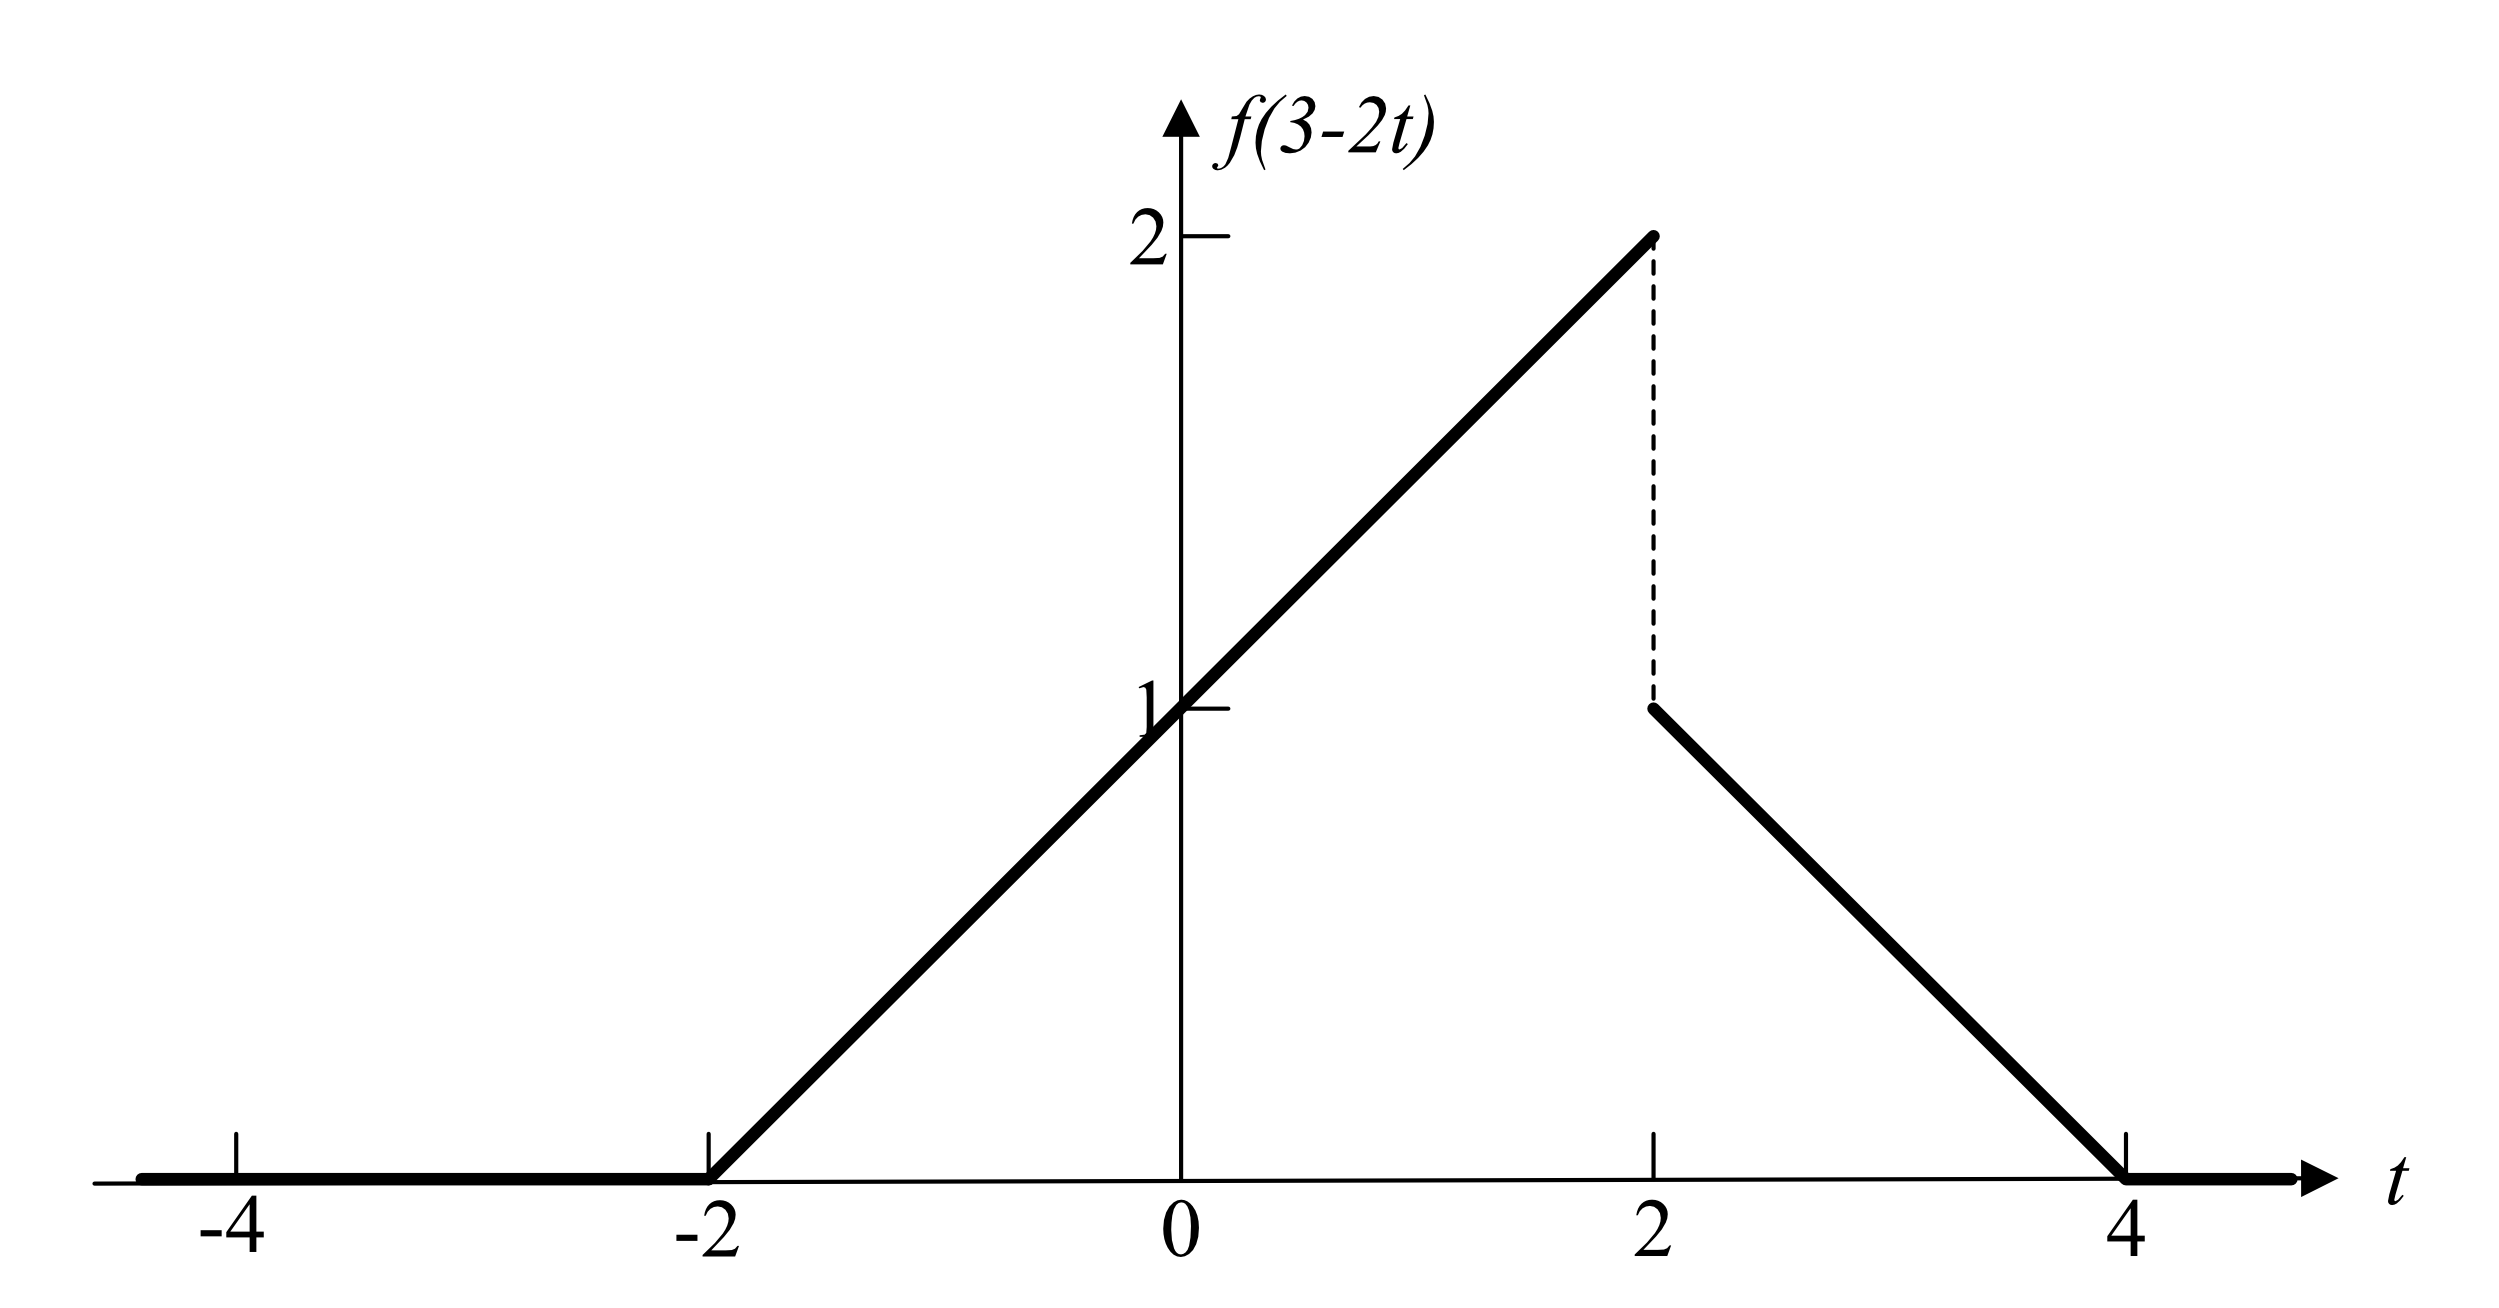
\includegraphics[width=8cm]{assets/hw1img3.png}
	\centering
\end{figure}
\quad
\end{problem}


































\end{document}